\documentclass[notitlepage,aps,prd,nofootinbib]{revtex4-1}

\usepackage{subfig}
%\usepackage[colorinlistoftodos]{todonotes}
\usepackage{float}

%\usepackage[protrusion=true,expansion=true]{microtype}
\usepackage{amsmath}
\usepackage{amssymb}
\usepackage{bbm}
\usepackage{ulem}
%\usepackage{feynmp-auto}
%\usepackage{slashed}
%\usepackage[absolute,overlay]{textpos}
\usepackage[usenames, dvipsnames]{color}
\usepackage{graphicx}
\usepackage{listings}
\usepackage{epsfig}
\usepackage{hyperref}
%\usepackage{tikz}
\usepackage{enumerate}
%\usepackage{fixltx2e} % buggy
\usepackage[compatibility=false]{caption}
%\usepackage{subcaption} % doesn't work with subfigure
\usepackage{pdfpages}
%\usepackage{setspace}
\usepackage{verbatim}

% Turn off meaningless float warnings
\usepackage{silence}
\WarningFilter{revtex4-1}{Repair the float}

\DeclareRobustCommand{\orderof}{\ensuremath{\mathcal{O}}}

\definecolor{dukeblue}{RGB}{0,0,156}
\definecolor{dukedarkblue}{RGB}{0,26,87}
\definecolor{dukeblack}{RGB}{79,79,79}
\definecolor{dukegray}{RGB}{79,79,79}
\definecolor{dukesecbrown}{RGB}{217,200,158}
\definecolor{dukesecblue}{RGB}{127,169,174}

%\renewcommand*{\thefootnote}{\fnsymbol{footnote}}

%%%%%%%%%%%%%%%%%%%%%%%%%%%%%%%%%%%%%%%%%%%%%%%%%%%%%%%%%%%%%%%%%%%%%%%%%%%%%%%%%%%%%
\hypersetup{
    breaklinks,
    baseurl       = http://,
    pdfborder     = 0 0 0,
    pdfpagemode   = UseNone,% do not show thumbnails or bookmarks on opening
    pdfstartpage  = 1,
    bookmarksopen = true,
    bookmarksdepth= 2,% to show sections and subsections
% revtex needs author and title declared after \begin{document}, so have to hard code them...
%    pdfauthor     = {\@author},
%    pdftitle      = {\@title},
    pdfauthor     = {Matthew Epland},
    pdftitle      = {Phys 566 Final},
    pdfsubject    = {},
    pdfkeywords   = {}}


% Code import settings
%%%%%%%%%%%%%%%%%%%%%%%%%%%%%%%%%%%%%%%%%%%%%%%%%%%%%%%%%%%%%%%%%%%%%%%%%%%%%%%%%%%%%
\definecolor{mygreen}{rgb}{0,0.6,0}
\definecolor{mygray}{rgb}{0.5,0.5,0.5}
\definecolor{mymauve}{rgb}{0.58,0,0.82}

%\lstset{ %
\lstdefinestyle{python}{ %
  backgroundcolor=\color{white},   % choose the background color; you must add \usepackage{color} or \usepackage{xcolor}
  basicstyle=\scriptsize,          % the size of the fonts that are used for the code
  breakatwhitespace=false,         % sets if automatic breaks should only happen at whitespace
  breaklines=true,                 % sets automatic line breaking
  captionpos=b,                    % sets the caption-position to bottom
  commentstyle=\color{mygreen},    % comment style
  deletekeywords={...},            % if you want to delete keywords from the given language
  escapeinside={\%*}{*)},          % if you want to add LaTeX within your code
  extendedchars=true,              % lets you use non-ASCII characters; for 8-bits encodings only, does not work with UTF-8
  frame=single,	                   % adds a frame around the code
  keepspaces=true,                 % keeps spaces in text, useful for keeping indentation of code (possibly needs columns=flexible)
  keywordstyle=\color{blue},       % keyword style
  language=Python,                 % the language of the code
  otherkeywords={*,...},           % if you want to add more keywords to the set
  numbers=left,                    % where to put the line-numbers; possible values are (none, left, right)
  numbersep=5pt,                   % how far the line-numbers are from the code
  numberstyle=\tiny\color{mygray}, % the style that is used for the line-numbers
  rulecolor=\color{black},         % if not set, the frame-color may be changed on line-breaks within not-black text (e.g. comments (green here))
  showspaces=false,                % show spaces everywhere adding particular underscores; it overrides 'showstringspaces'
  showstringspaces=false,          % underline spaces within strings only
  showtabs=false,                  % show tabs within strings adding particular underscores
  stepnumber=5,                    % the step between two line-numbers. If it's 1, each line will be numbered
  stringstyle=\color{mymauve},     % string literal style
  tabsize=2,	                   % sets default tabsize to 2 spaces
%  title=\lstname                   % show the filename of files included with \lstinputlisting; also try caption instead of title
  title={\protect\filename@parse{\lstname}\protect\filename@base.\filename@ext},
  firstnumber=0,
%  linewidth=0.95\textwidth
  xleftmargin=0.01\textwidth,
  xrightmargin=0.01\textwidth
}

\lstdefinestyle{output}{ %
  backgroundcolor=\color{white},   % choose the background color; you must add \usepackage{color} or \usepackage{xcolor}
  basicstyle=\scriptsize,          % the size of the fonts that are used for the code
  breakatwhitespace=false,         % sets if automatic breaks should only happen at whitespace
  breaklines=true,                 % sets automatic line breaking
  captionpos=b,                    % sets the caption-position to bottom
  escapeinside={\%*}{*)},          % if you want to add LaTeX within your code
  frame=single,	                   % adds a frame around the code
  keepspaces=true,                 % keeps spaces in text, useful for keeping indentation of code (possibly needs columns=flexible)
  numbers=left,                    % where to put the line-numbers; possible values are (none, left, right)
  numbersep=5pt,                   % how far the line-numbers are from the code
  numberstyle=\tiny\color{mygray}, % the style that is used for the line-numbers
  rulecolor=\color{black},         % if not set, the frame-color may be changed on line-breaks within not-black text (e.g. comments (green here))
  stepnumber=5,                    % the step between two line-numbers. If it's 1, each line will be numbered
  tabsize=2,	                   % sets default tabsize to 2 spaces
%  title=\lstname                   % show the filename of files included with \lstinputlisting; also try caption instead of title
  title={\protect\filename@parse{\lstname}\protect\filename@base.\filename@ext},
  firstnumber=0,
%  linewidth=0.95\textwidth
  xleftmargin=0.01\textwidth,
  xrightmargin=0.01\textwidth
}

\newcommand{\degree}{\ensuremath{^{\circ}}}

% Select between raw and saved plots here
%\graphicspath{{../output/}}

%%%%%%%%%%%%%%%%%%%%%%%%%%%%%%%%%%%%%%%%%%%%%%%%%%%%%%%%%%%%%%%%%%%%%%%%%%%%%%%%%%%%%
\begin{document}

\title{PHYS 566 Final}
\author{Matthew Epland}
\affiliation{Department of Physics, Duke University, Durham, NC 27707, USA}

\date{\today}

\begin{abstract}
In this assignment the Ising model was successfully simulated in 2D via the Metropolis algorithm, producing $M$ vs. $T$, $C/N$ vs. $T$, and $C_{\mathrm{max}}/N$ vs. $n$ curves. A spontaneous magnetization phase transition was observed in $M\left(T\right)$, and $C_{\mathrm{max}}/N$ was found to scale like $\sim \log(n)$ for small values of $n$, both of which match the expected behaviors of the model.
\end{abstract}\maketitle

\section{Introduction and Theory}
\label{sec:theory}
\subsection{Ising Model}
\label{subsec:ising}
The Ising model is the standard statistical mechanics first order model for a lattice of spins, such as the spins of atoms in a ferromagnet. It is unique in being both analytically solvable, for some cases\footnote{1D with periodic boundary conditions is fairly straight forward, however no 3D analytical solutions have yet been developed.}, and in having a phase transition. In the Ising model each lattice point can either be spin up, $s=+1$ or spin down, $s=-1$, and the Hamiltonian\footnote{Without the presence of an external field} (\ref{eq:E}) only considers nearest neighbor (NN) interactions with exchange energy $J$.

\begin{equation}
\label{eq:E}
E = -J \sum_{\mathrm{NN}} s_{i} s_{j}
\end{equation}

Due to the binary spin orientations, the magnetization of an Ising model lattice can easily be calculated as a simple average over the $N$ lattice points (\ref{eq:M}).

\begin{equation}
\label{eq:M}
M = \frac{1}{N} \sum_{j=1}^{N} s_{i} = N \langle s \rangle
\end{equation}

The above equations apply to specific lattices or microstates. As is common in statistical mechanics we can take averages over microstates $\alpha$ to produce more accurate thermal quantities, in particular $\langle E \rangle$ (\ref{eq:ave_E}) and $\langle E^{2} \rangle$ (\ref{eq:ave_E2}).

\begin{align}
\langle E \rangle &= \frac{1}{N_{\mathrm{microstates}}} \sum_{\alpha} E_{\alpha} \label{eq:ave_E} \\
\langle E^{2} \rangle &= \frac{1}{N_{\mathrm{microstates}}} \sum_{\alpha} E_{\alpha}^{2} \label{eq:ave_E2}
\end{align}

We are interested in $\langle E \rangle$ and $\langle E^{2} \rangle$ because they can be used to compute the squared variance of $E$, $\sigma_{E}^{2}$ (\ref{eq:sigmaE2}), which can itself be used to compute the specific heat $C$ at temperature $T$ via the fluctuation--dissipation theorem\footnote{$k_{B}$ is the standard Boltzmann constant.} (\ref{eq:C}).

\begin{align}
\sigma_{E}^{2} &=  \langle E^{2} \rangle - \langle E \rangle^{2} \label{eq:sigmaE2} \\
C &= \frac{\sigma_{E}^{2}}{k_{B} T^{2}} \label{eq:C}
\end{align}

The Ising model can exhibit a phase transition between $M=\langle s \rangle \sim 0$ disordered spins and $\left|M\right|\sim N,\,\left|\langle s \rangle\right| \sim 1$ ordered spins, ie spontaneous magnetization, as $T$ changes through some critical $T_{C}$. It is possible to analytically derive $T_{C}$, and indeed this is one of the Ising models main positives, however we will not be discussing analytical approaches in this work.\footnote{References can easily be found in the literature, one example is Pathria and Beale.} Instead we will be focused on simulating the Ising model numerically with the Metropolis algorithm.

\subsection{Metropolis Algorithm}
\label{subsec:met_alg}

The Ising model is an ideal candidate for Monte Carlo simulation as it only depends on nearest neighbor interactions. The Metropolis algorithm is one Monte Carlo technique for modeling such interactions on an $n\times n$ lattice, $N=n^{2}$, with periodic boundary conditions. The algorithm assumes the lattice is held at temperature $T$ by an external heat bath. In this work $n=5$ to $500$, $J=1.5$ J, and $k_{B}=1$ J/K were used, setting the interesting temperature range to be around $0 < T < 5$ K. The nearest neighborhood type chosen is for use in the Metropolis algorithm is typically either the Von Neumann or Moore neighborhood\footnote{The Von Neumann neighborhood consists of the four normal lattice points; left, right, up, and down, of the original point. The Moore neighborhood adds the four diagonal neighbors for a total of eight.}. The Von Neumann neighborhood was chosen for use in this work, though the simulation code was written such that either neighborhood type could be easily selected.to be able to use either.

The Metropolis algorithm begins by initializing the lattice as an $n\times n$ array of randomly generated spins, $\pm 1$. Sweeps are performed of the array\footnote{The sweeps of the lattice can be done by going through the lattice points sequentially or randomly. Here the simpler sequential option was used.} changing each lattice point's spin according to the following rules. First the spin is flipped and $\Delta E = E_{\mathrm{flipped}} - E_{\mathrm{original}}$ is computed. Note that due to the structure of the Hamiltonian (\ref{eq:E}) $\Delta E$ only depends on the spin's NN points and thus is an easy sum to perform computationally. If $\Delta E \leq 0$ the flipped spin will always be kept and the sweep moves on to the next point. If $\Delta E > 0$ the flipped spin will be kept with probability $p$ (\ref{eq:p}) as a function of $\Delta E$ and $T$, but otherwise will be flipped a second time returning to its original state. This chance of changing the spin to an energetically unfavorable state models the random thermal excitations of the atoms, which naturally die away as $T\rightarrow0$ thereby producing the $\langle s \rangle \rightarrow \pm 1$ spontaneous magnetization behavior.

Sweeps are performed of the lattice in this manner until a halting condition is met, at which point the thermodynamic properties of the lattice, such as $E$ and $M$, can be computed. Due to the large number of sweeps, through a potentially $N=n^2$ large number of lattice points, a compiled C module was written to perform sweeps and compute $E$ in order to decrease the overall Python code's run time.




\begin{equation}
\label{eq:p}
p = \exp\left(\frac{-\Delta E}{k_{B} T}\right)
\end{equation}

\subsubsection{Halting Conditions and Convergence}
\label{subsubsec:convergence}
While the Metropolis algorithm does find equilibrium solutions it does not necessarily converge monotonically to equilibrium. To prevent a single random fluctuation from halting the simulation prematurely, the average of the percent absolute change in energy between sweeps $\langle \Delta E / E \rangle$ (\ref{eq:histE}) over the past $N_{\mathrm{history}} = 10$ sweeps was used to judge convergence. The simulation was written to stop sweeping when $\langle \Delta E / E \rangle < 0.01$, or when the number of sweeps reached an upper limit, $N_{\mathrm{sweeps}} = 10000$ or $20000$. The $\langle \Delta E / E \rangle < 0.01$ halting condition always resulted in an equilibrium lattice. The $N_{\mathrm{sweeps}}$, time out halting condition in general does not guarantee an equilibrium lattice, however the upper limit on the number of sweeps was set large enough that in effect semi--equilibrium states were found\footnote{Semi--equilibrium meaning that the total energy is still fluctuating but $\langle s \rangle$ and the general $\pm1$ regions of the lattice are roughly constant. The simulation tended to time out at higher $T$s, where there is more thermal fluctuation, and lower $n$.}.


\begin{equation}
\label{eq:histE}
\langle \Delta E / E \rangle \equiv \frac{1}{N_{\mathrm{history}}} \sum_{i=1}^{N_{\mathrm{history}}} \left|\frac{ E_{i+1} - E_{i}}{E_{i+1}}\right|
\end{equation}


\clearpage
\section{Results}
\label{sec:results}

\subsection{Part A}
\label{subsec:results_part_a}
In the first half of the assignment we are interested in the behavior of $M$ as a function of $T$, particularly the spontaneous magnetization phase transition and $T_{C}$. To investigate this behavior we cool a $n=50$ lattice down in stages from $T=9$ to $0.1$ K, using the equilibrium or halting array from one $T$ as the starting array for the next $T$. The temperatures investigated\footnote{$T = 0.1, 0.5, 1, 1.5, 2, 2.25, 2.5, 2.6, 2.7, 2.8, 2.9, 3, 3.1, 3.2, 3.3, 3.35, 3.4, 3.45, 3.5, 3.55, 3.6, 3.7, 3.8, 3.9, 4, 4.5, 5, 5.5, 6, 6.5, 7, 8, 9$} where chosen by hand to minimize the total run time while still showing the phase transition and general behavior in detail. The initial randomly generated lattice and equilibrium lattices at a few example $T$s are shown in Figures~\ref{fig:initial} through~\ref{fig:T2.5} below. As mentioned previously, the higher $T$ lattices did not satisfy the convergence condition, but were in reasonable semi--equilibrium states when the simulation timed out at $N_{\mathrm{sweeps}} = 20000$. The resulting plot of $M/N$ vs. $T$, Figure~\ref{fig:M_vs_T}, shows a nice spontaneous magnetization phase transition from $\langle s \rangle = 0$ to $\langle s \rangle = +1$ at a critical temperature\footnote{$T_{C}$ was determined graphically by hand.} of $T_{C} = 3.50$ K, matching our phenomenological expectations.

\begin{figure}[!htbc]
  \centering
  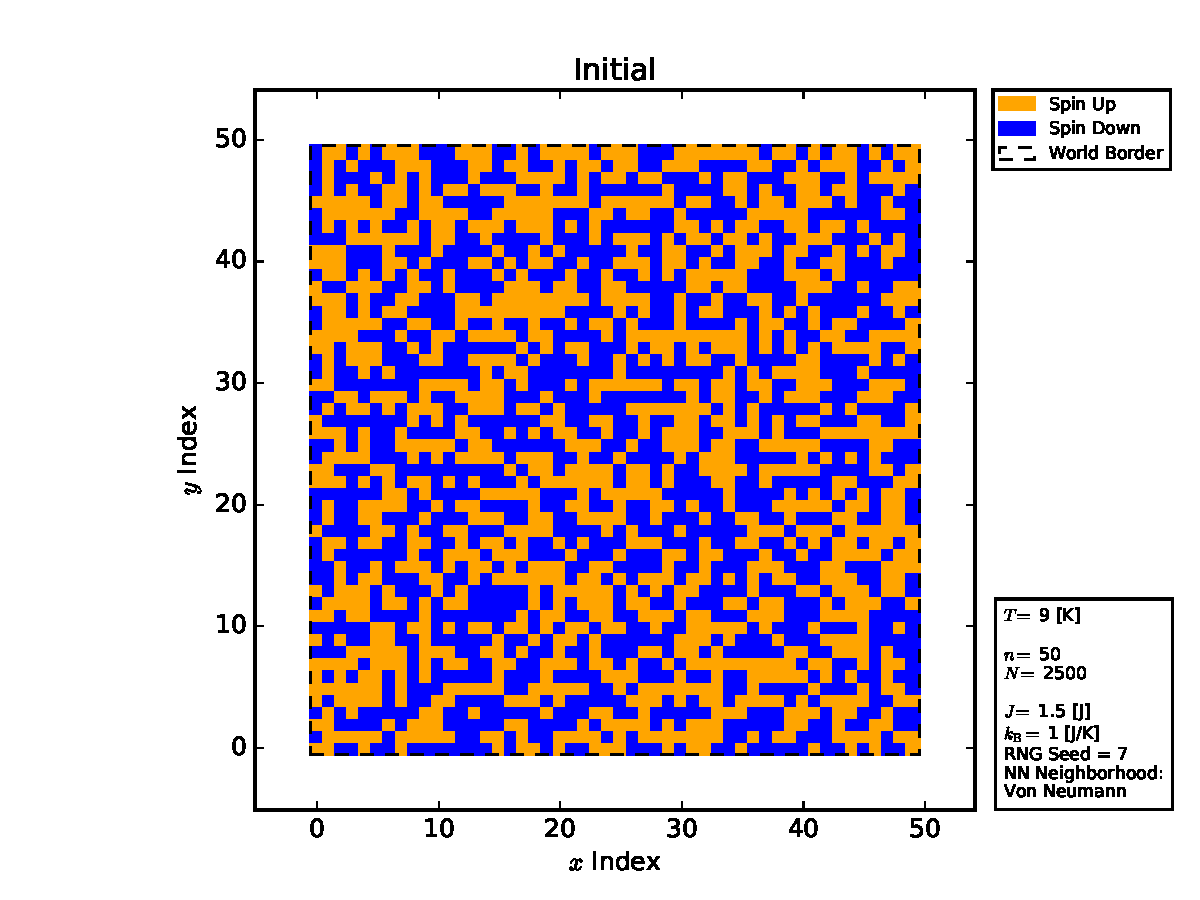
\includegraphics[width=.82\textwidth]{../output/plots_for_paper_von_neumann/part_a/initial.pdf}
	{\par\nobreak\rule[9pt]{35em}{0.5pt}\vspace{-5mm}}
	\caption{Initial lattice.}
	\label{fig:initial}
\end{figure}

\clearpage
\begin{figure}[!htbc]
  \centering
  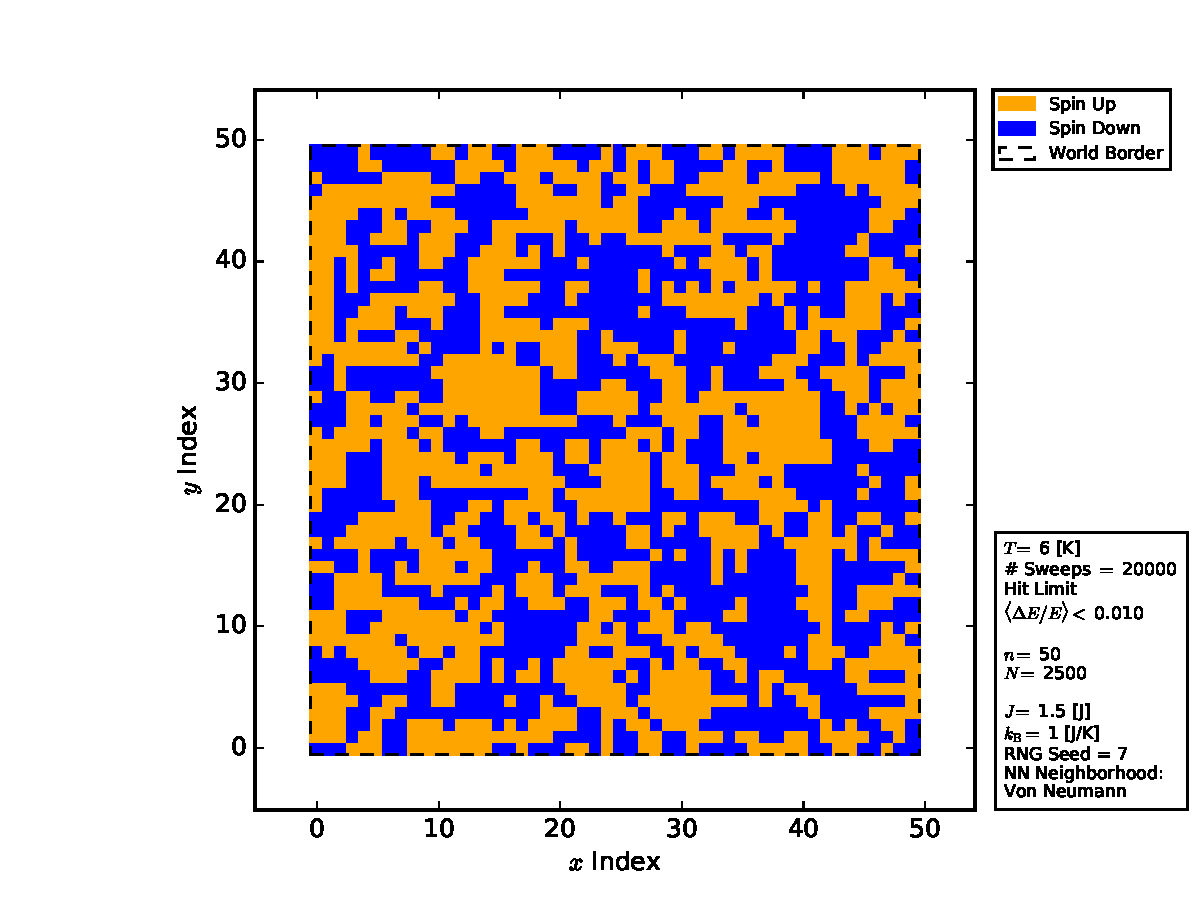
\includegraphics[width=.75\textwidth]{{../output/plots_for_paper_von_neumann/part_a/converged_T6.00}.pdf}
	{\par\nobreak\rule[9pt]{35em}{0.5pt}\vspace{-5mm}}
	\caption{Lattice at $T=6.0$. While the convergence condition was not met before the simulation timed out the lattice seems reasonable.}
	\label{fig:T6.0}
\end{figure}

\begin{figure}[!htbc]
  \centering
  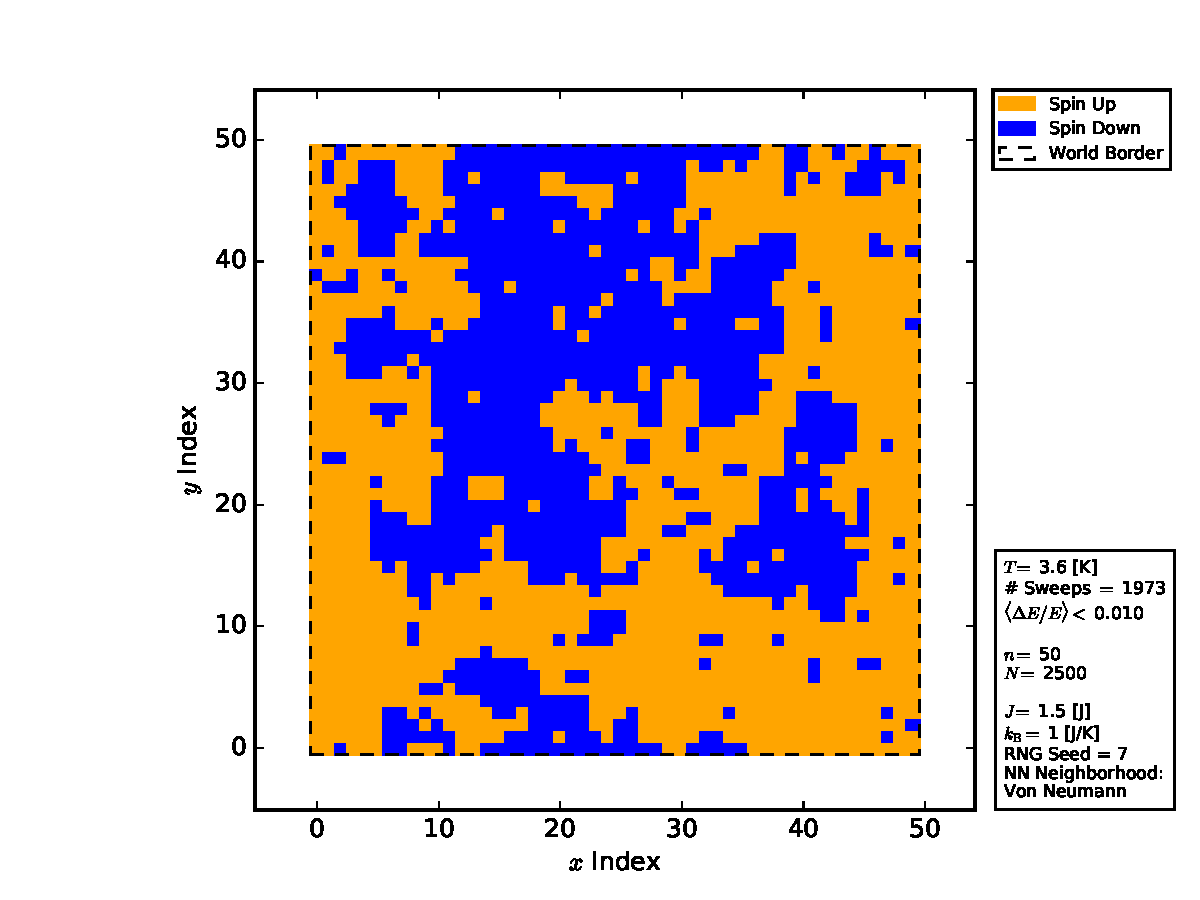
\includegraphics[width=.75\textwidth]{{../output/plots_for_paper_von_neumann/part_a/converged_T3.60}.pdf}
	{\par\nobreak\rule[9pt]{35em}{0.5pt}\vspace{-5mm}}
	\caption{Lattice at $T=3.6$. Here the simulation met the convergence condition.}
	\label{fig:T3.6}
\end{figure}

\clearpage
\begin{figure}[!htbc]
  \centering
  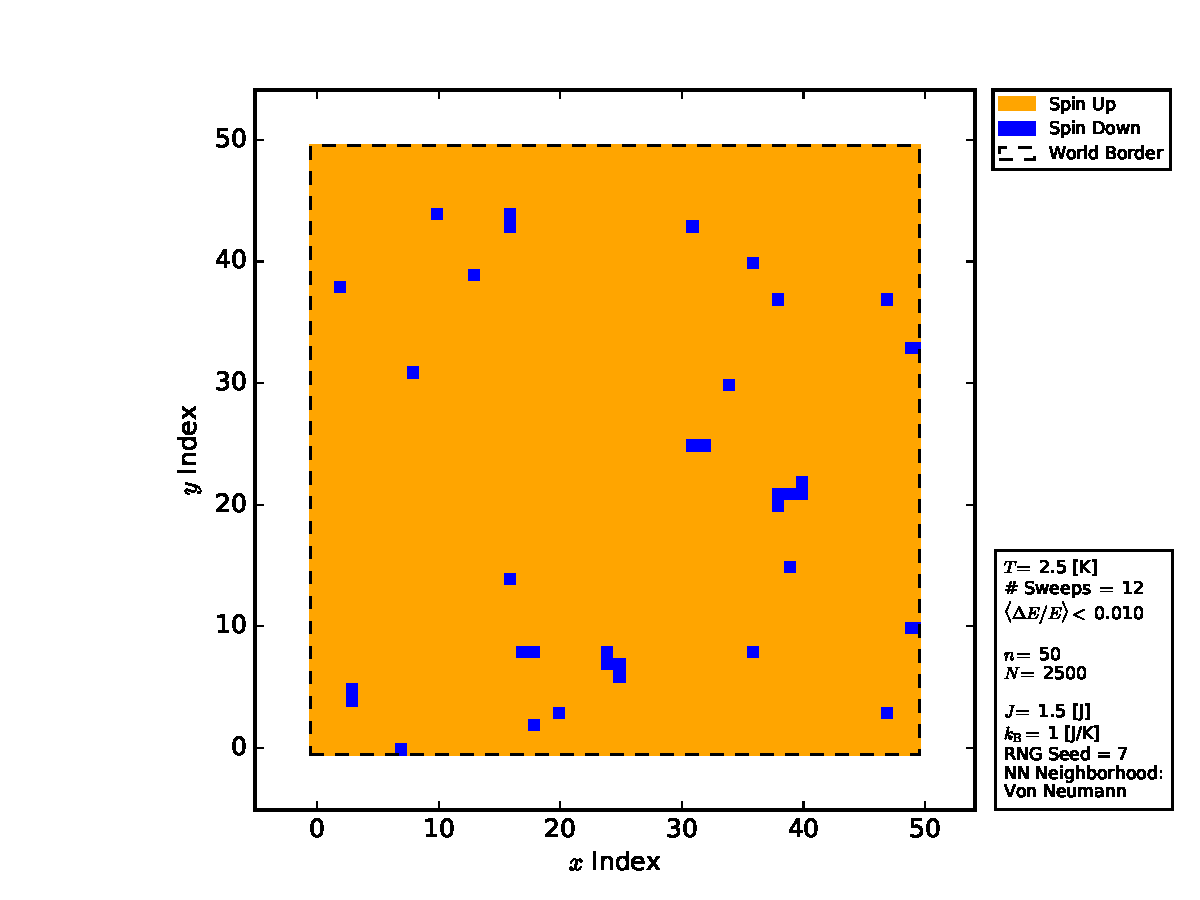
\includegraphics[width=.75\textwidth]{{../output/plots_for_paper_von_neumann/part_a/converged_T2.50}.pdf}
	{\par\nobreak\rule[9pt]{35em}{0.5pt}\vspace{-5mm}}
	\caption{Lattice at $T=2.5$. At lower $T$ the lattice becomes increasingly uniform.}
	\label{fig:T2.5}
\end{figure}

\begin{figure}[!htbc]
  \centering
  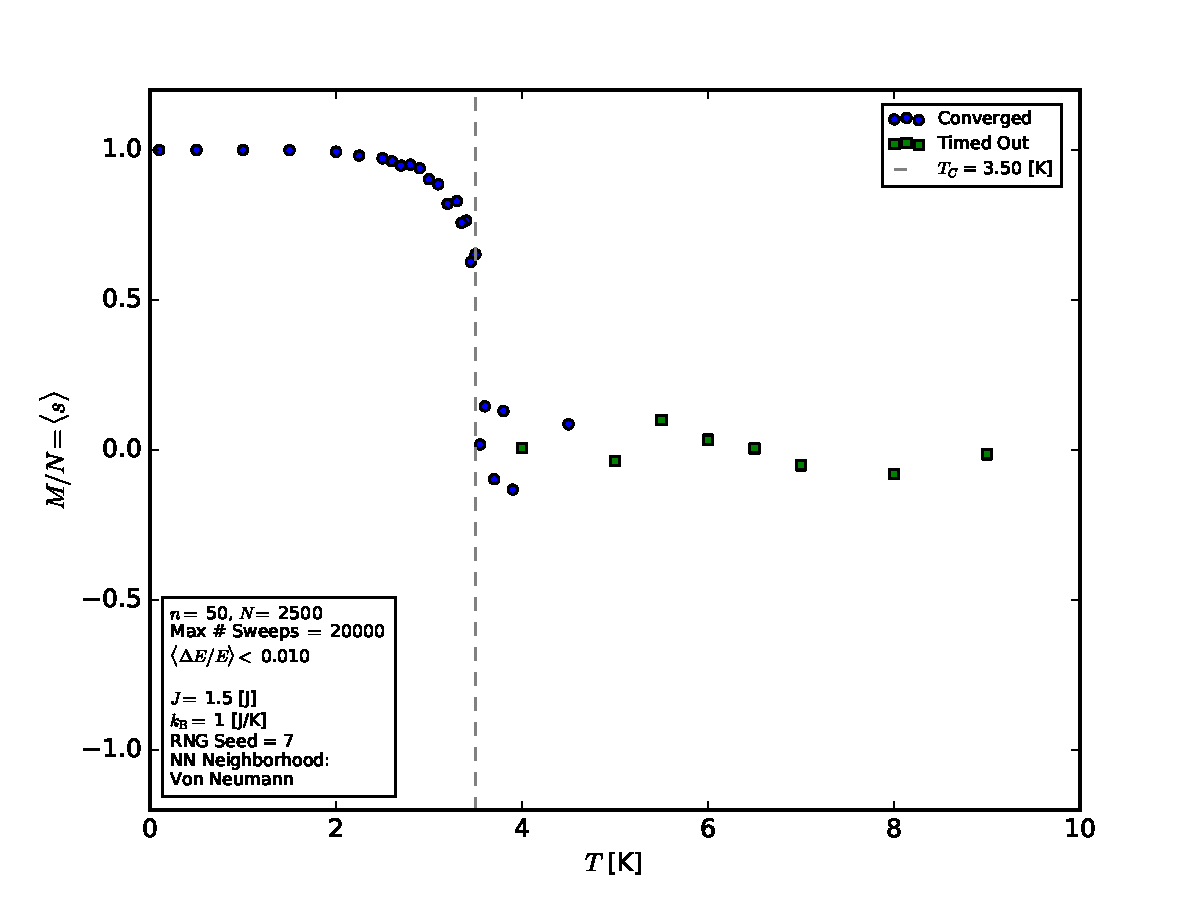
\includegraphics[width=.75\textwidth]{../output/plots_for_paper_von_neumann/part_a/M_vs_T.pdf}
	{\par\nobreak\rule[9pt]{35em}{0.5pt}\vspace{-5mm}}
	\caption{$M/N$ vs. $T$. Notice the phase transition between $\langle s \rangle = 0$ and $\left|\langle s \rangle\right| = 1$ at $T_{C} = 3.50$ K. For this simulation and RNG seed the lattice transitioned to the $\langle s \rangle = 1$ spin up magnetization state.}
	\label{fig:M_vs_T}
\end{figure}



\clearpage
\subsection{Part B}
\label{subsec:results_part_b}
In the second half of the assignment we turn our focus to the specific heat $C$ as a function of lattice size $n$. To allow us to compare $C$ between different $n$ values we must divide by the total number of lattice points $N$. $C/N$ can be calculated via the fluctuation--dissipation theorem, but first we must compute $\sigma_{E}^{2}$ which involves averaging over many microstates of a single macrostate. To generate these microstates it is not necessary to start from a random initial lattice like Figure~\ref{fig:initial} every time, but instead one initial state can be simulated to equilibrium at $T$, then the rest of the microstates can be generated from the equilibrium lattice by simply preforming more sweeps on it. In this assignment $N_{\mathrm{microstates}} = 100$ microstates, each separated by 10 full lattice sweeps, were used to generate each $\sigma_{E}^{2}$, and hence $C/N$, value. Using these method $C/N$ vs. $T$ curves\footnote{$T = 2.0, 2.5, 2.9, 3.0, 3.1, 3.2, 3.3, 3.4, 3.5, 3.6, 3.7, 3.8, 3.9, 4.0, 4.1, 4.2, 4.3, 4.4, 4.5, 5.0$} were generated for a variety of $n$ values\footnote{$n = 5, 10, 20, 30, 40, 50, 75, 100, 200, 500$}, see Figures~\ref{fig:CT_n10} through~\ref{fig:CT_n500}. Due to the very large number of sweeps needed to complete this task it was necessary to implement the compiled C module. Additionally $N_{\mathrm{sweeps}}$ was reduced\footnote{In fact this was the original value and $N_{\mathrm{sweeps}}$ was bumped up for part A as the lower number of sweeps required made it possible to do so.} to $10000$.

From each of the $C/N$ vs. $T$ plots we can find a maximum $C_{\mathrm{max}}$ allowing us to plot $C_{\mathrm{max}}$ vs. $n$. From the problem assignment we expect to see $C_{\mathrm{max}}\left(n\right)$ obey an approximate finite--size scaling relation $C_{\mathrm{max}}/N \sim \log(n)$, particularly for small values of $n$. Indeed looking at the linear fit of  $C_{\mathrm{max}}/N$ vs. $\log(n)$ in Figure~\ref{fig:Cmax_over_N_vs_n} we see that the simulated data is consistent with the scaling relation, $C_{\mathrm{max}}/N = -0.33 + 3.37 \log(n)$ for $n < 60$.


\begin{figure}[!htbc]
  \centering
  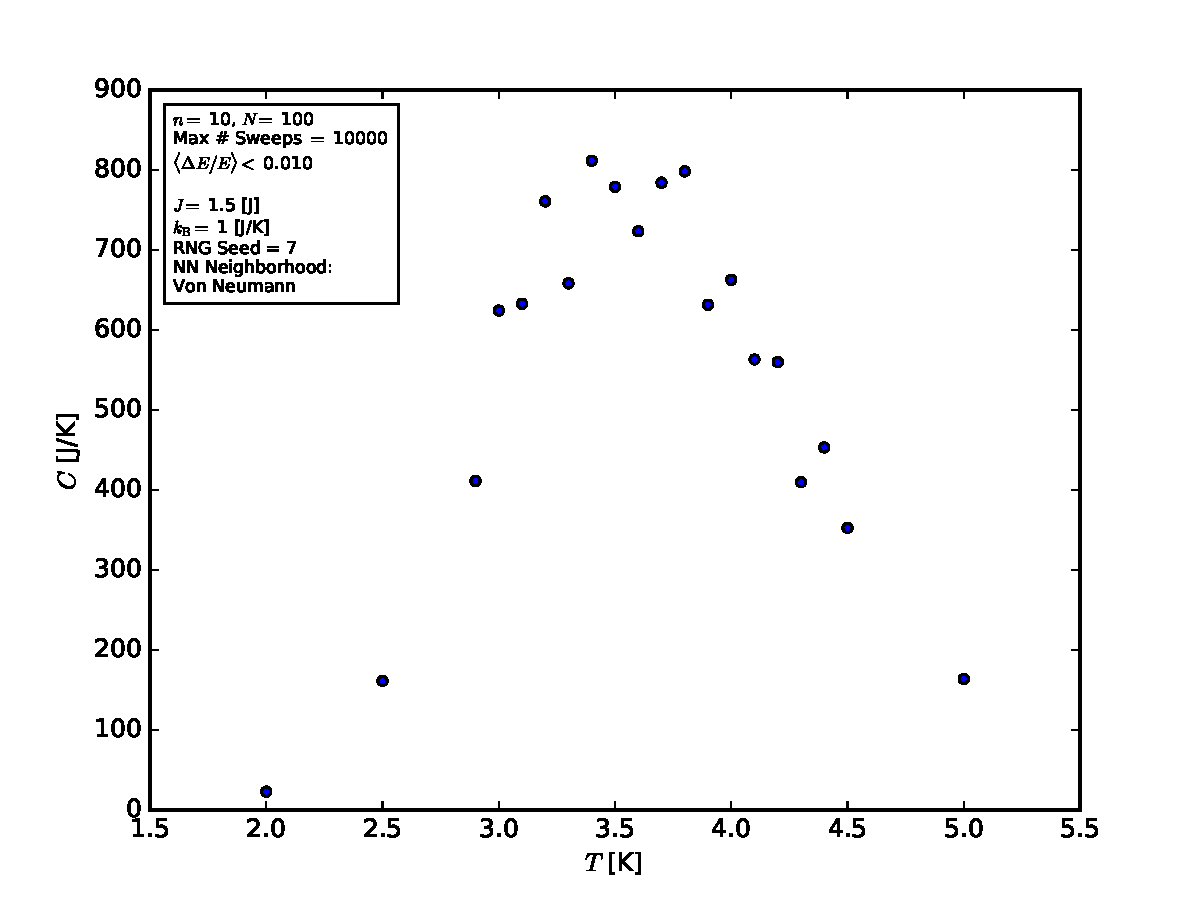
\includegraphics[width=.8\textwidth]{../output/plots_for_paper_von_neumann/part_b/CT_for_n10.pdf}
	{\par\nobreak\rule[9pt]{35em}{0.5pt}\vspace{-5mm}}
	\caption{$C\left(T\right)$ for $n=10$. This is an example of the noise present at low $n$.}
	\label{fig:CT_n10}
\end{figure}

\clearpage
\begin{figure}[!htbc]
  \centering
  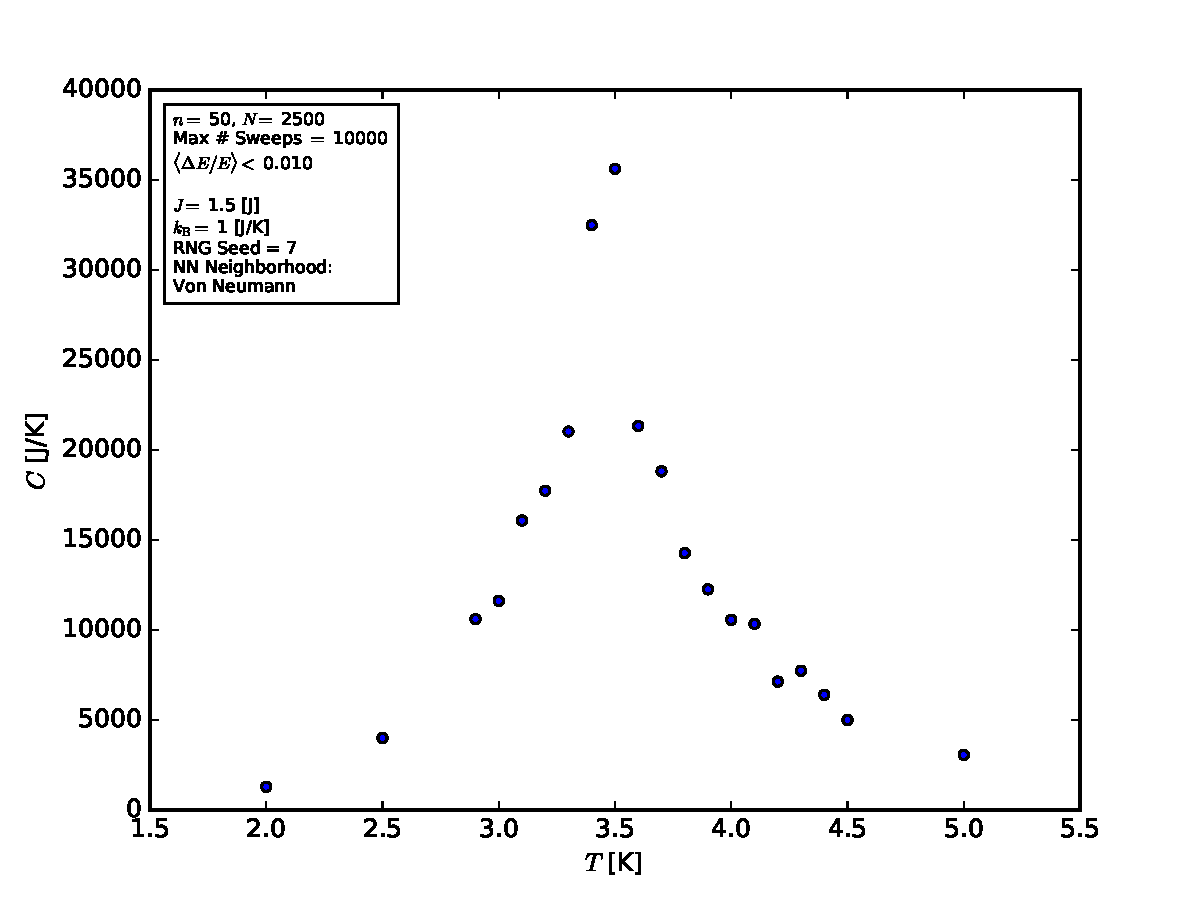
\includegraphics[width=.75\textwidth]{../output/plots_for_paper_von_neumann/part_b/CT_for_n50.pdf}
	{\par\nobreak\rule[9pt]{35em}{0.5pt}\vspace{-5mm}}
	\caption{$C\left(T\right)$ for $n=50$. This $n$ value produced the sharpest peak in $C\left(T\right)$.}
	\label{fig:CT_n50}
\end{figure}

\begin{figure}[!htbc]
  \centering
  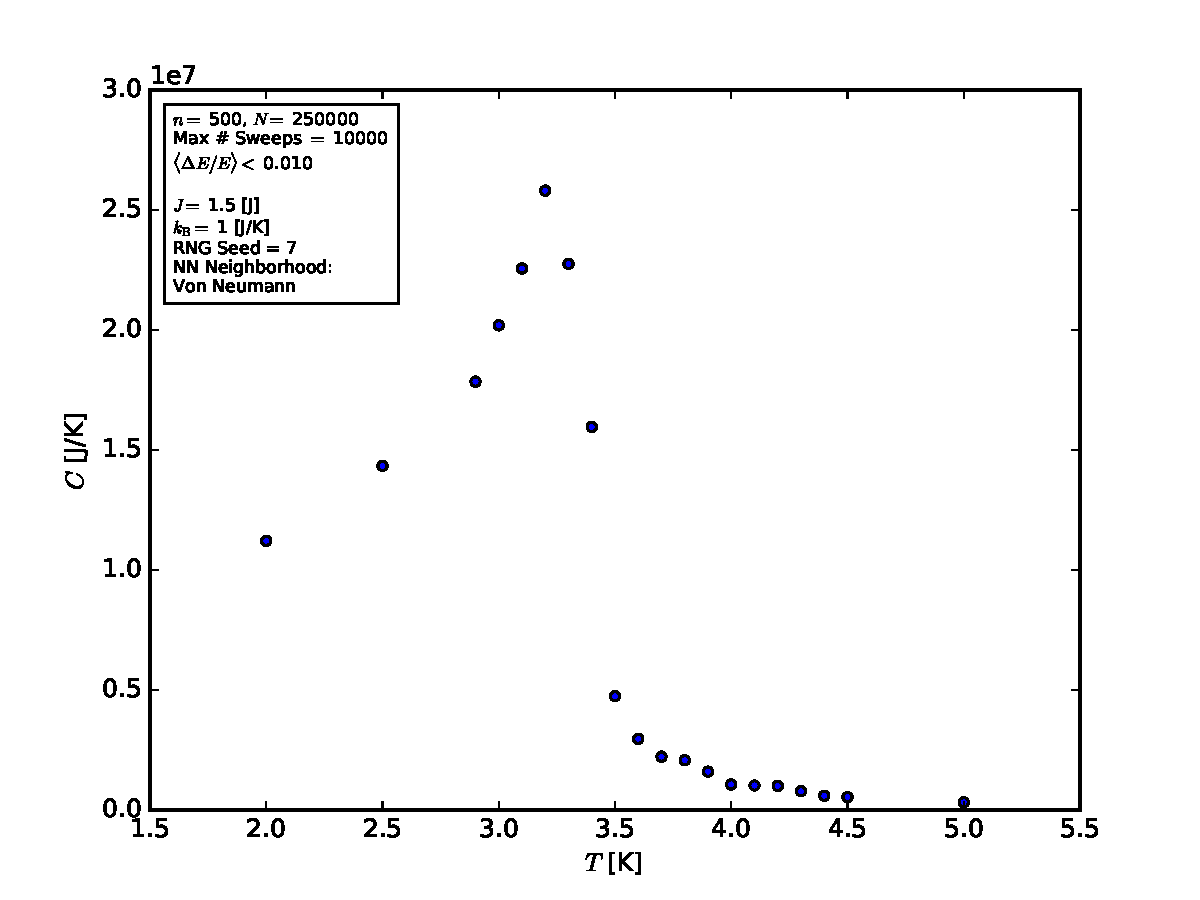
\includegraphics[width=.75\textwidth]{../output/plots_for_paper_von_neumann/part_b/CT_for_n500.pdf}
	{\par\nobreak\rule[9pt]{35em}{0.5pt}\vspace{-5mm}}
	\caption{$C\left(T\right)$ for $n=500$.}
	\label{fig:CT_n500}
\end{figure}


\clearpage
\begin{figure}[!htbc]
  \centering
  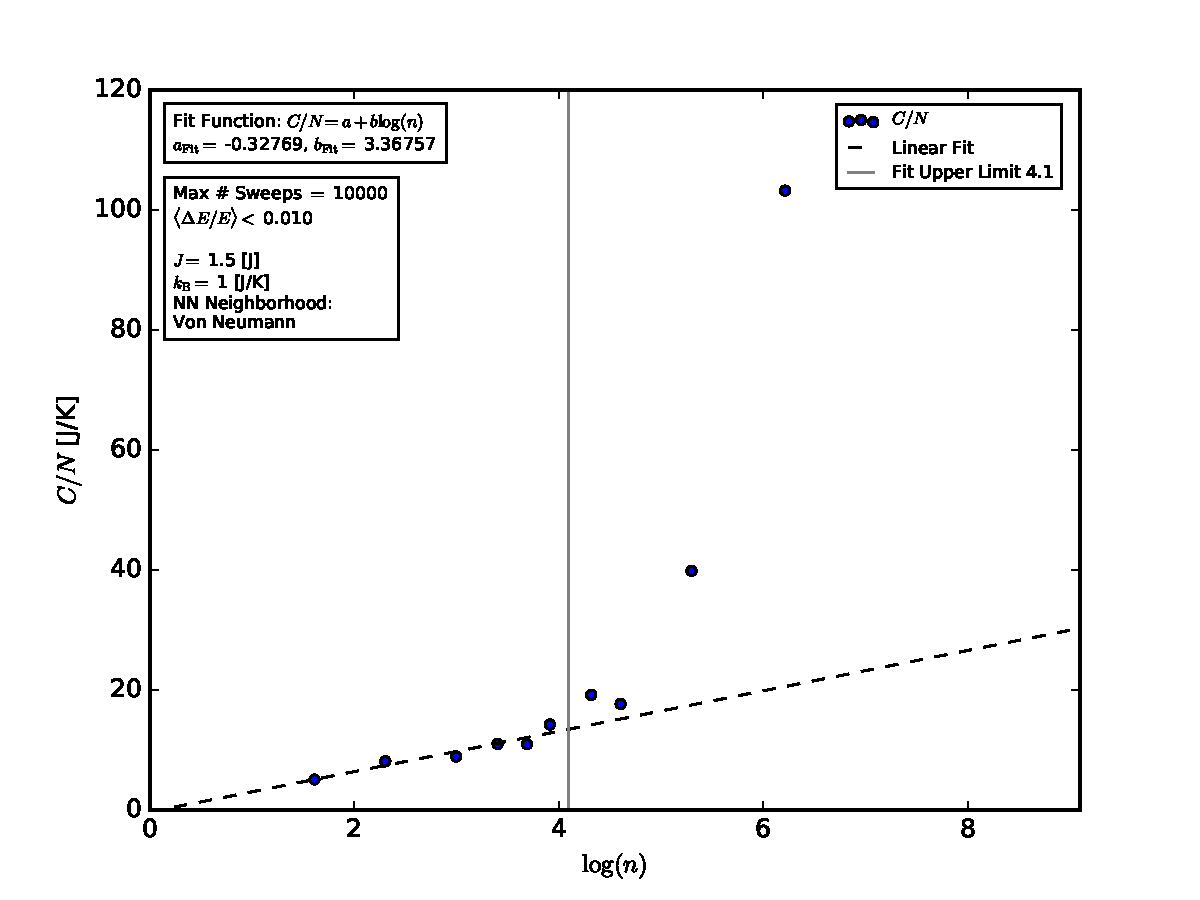
\includegraphics[width=.82\textwidth]{../output/plots_for_paper_von_neumann/part_b/Cmax_over_N_vs_n.pdf}
	{\par\nobreak\rule[9pt]{35em}{0.5pt}\vspace{-5mm}}
	\caption{$C_{\mathrm{max}}/N$ vs. $\log(n)$. The linear fit is consistent with $C_{\mathrm{max}}/N \sim \log(n)$, for low $n$.}
	\label{fig:Cmax_over_N_vs_n}
\end{figure}


\section{Conclusions}
\label{sec:Conclusions}
The Ising model in 2D was successfully simulated via the Metropolis algorithm. A $M\left(T\right)$ curve with a spontaneous magnetization phase transition was generated for a lattice of $n=50$. $C/N$ vs. $T$, and $C_{\mathrm{max}}/N$ vs. $n$ curves were also generated that showed scaling like $C_{\mathrm{max}}/N \sim \log(n)$ for small values of $n$. All of these results agreed with the expected behavior of the Ising model.

The Python and C source code used to produce these results can be found online at \url{http://github.com/mepland/PHYS_566_Computational_HW/tree/master/final/code}, and is included in Section~\ref{sec:code}.


\clearpage
\section{Supporting Material}
\label{sec:Supporting_Material}

\lstinputlisting[style=output,label={lst:output_part_a}]{../output/plots_for_paper_von_neumann/part_a/part_a.log}
\lstinputlisting[style=output,label={lst:output_part_b}]{../output/plots_for_paper_von_neumann/part_b/part_b.log}


\clearpage
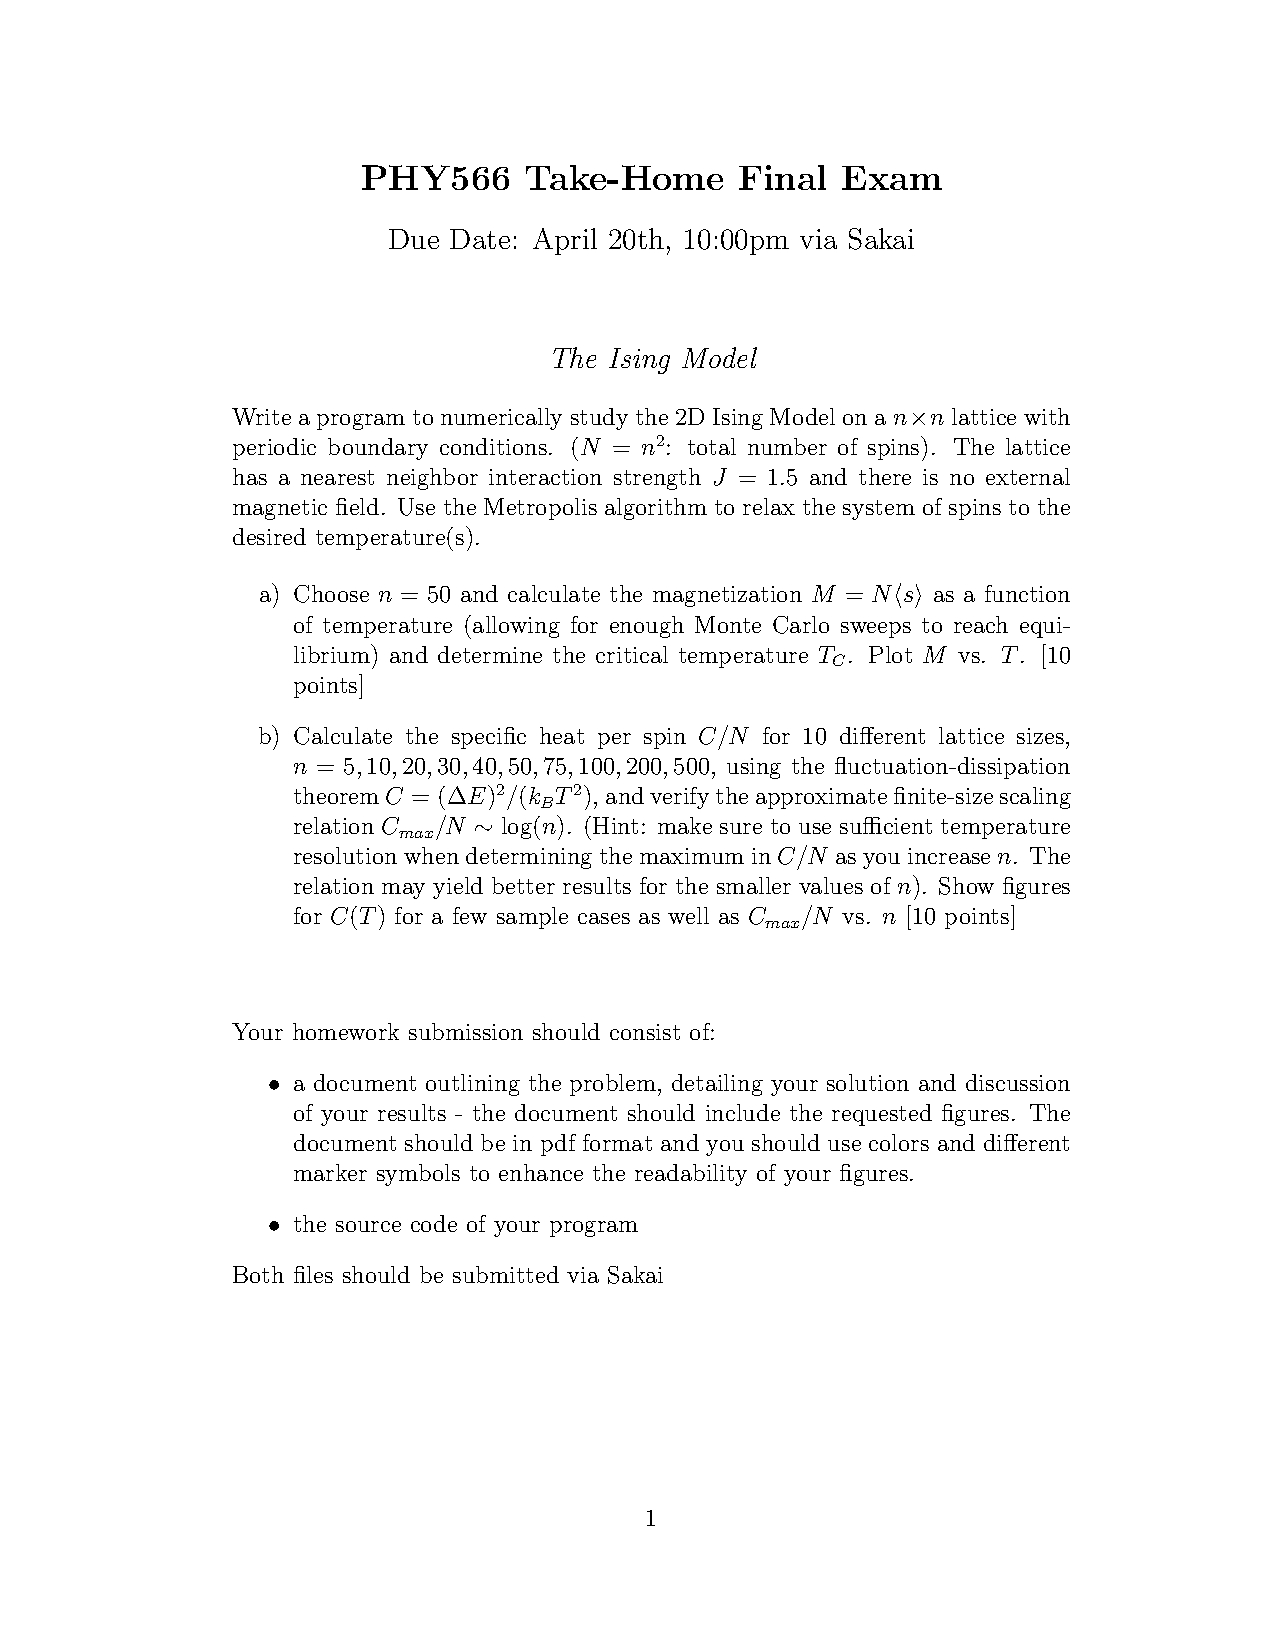
\includepdf{../final.pdf}

\clearpage
\section{Code}
\label{sec:code}

\lstinputlisting[style=python]{../code/metropolis_ising.py}
\lstinputlisting[style=python]{../code/sweepmodule.c}
\lstinputlisting[style=python]{../code/module_setup_for_sweepMod.py}

\end{document} %%% end of doc %%%
%%%%%%%%%%%%%%%%%%%%%%%%%%%%%%%%%%%%%%%%%%%%%%%%%%%%%


\bibliographystyle{bib_files/styles/atlasBibStyleWoTitle}
\bibliography{bib_files/my_bib.bib}


